\documentclass[border=3pt]{standalone}
% Preâmbulo compartilhado pelos diagramas TikZ da aula 13 (SLAM com EKF)
\usepackage[T1]{fontenc}
\usepackage[utf8]{inputenc}
\usepackage{lmodern}
\usepackage{amsmath}
\usepackage{xcolor}
\usepackage{tikz}
\usetikzlibrary{arrows.meta,angles,quotes,decorations.pathmorphing,decorations.pathreplacing,calc,
                positioning,shapes.geometric,shapes.misc,backgrounds,fit,
                math}

% Paleta (mesma dos SVGs originais)
\definecolor{dblue}{HTML}{2A5B8C}
\definecolor{dorange}{HTML}{B3541E}
\definecolor{dgreen}{HTML}{4A7C59}
\definecolor{dred}{HTML}{9C4B4B}
\definecolor{dcream}{HTML}{F4F1EA}
\definecolor{dshade}{HTML}{DDD7C9}

% Função gaussiana (não normalizada por padrão de escala visual)
\pgfmathdeclarefunction{gauss}{3}{%
  \pgfmathparse{1/(#3*sqrt(2*pi))*exp(-((#1-#2)^2)/(2*#3^2))}%
}

% Estilos comuns (prefixo d... para não colidir com chaves internas do pgf)
\tikzset{
  >={Stealth[length=2mm]},
  dguide/.style={gray!55, dashed, line width=0.4pt},
  daxis/.style={gray!60, line width=0.7pt, ->},
  dbody/.style={fill=black!3, draw=black!80, line width=1pt},
  dacc/.style={draw=dblue, line width=1pt},
  dlbl/.style={black!55, font=\small},
  dsub/.style={black!45, font=\footnotesize},
  dstate/.style={circle, draw=black!80, fill=dcream, line width=1pt,
                 minimum size=17mm, font=\large, inner sep=1pt},
  dobs/.style={circle, draw=black!80, fill=dshade, line width=1pt,
               minimum size=14mm, font=\large, inner sep=1pt},
  dbox/.style={rounded corners=2pt, draw=black!80, fill=dcream, line width=1pt,
               align=center, inner sep=6pt},
  dop/.style={circle, draw=black!80, fill=white, line width=1pt,
              minimum size=6mm, inner sep=0pt, font=\small},
  dtrans/.style={->, dblue, line width=1pt},
  dmeas/.style={->, dorange, line width=1pt},
  dcurve/.style={line width=1pt, dblue},
  dcurveb/.style={line width=1.4pt, dorange},
}

\begin{document}
\hyphenpenalty=10000 \exhyphenpenalty=10000 \tolerance=9999 \emergencystretch=3em
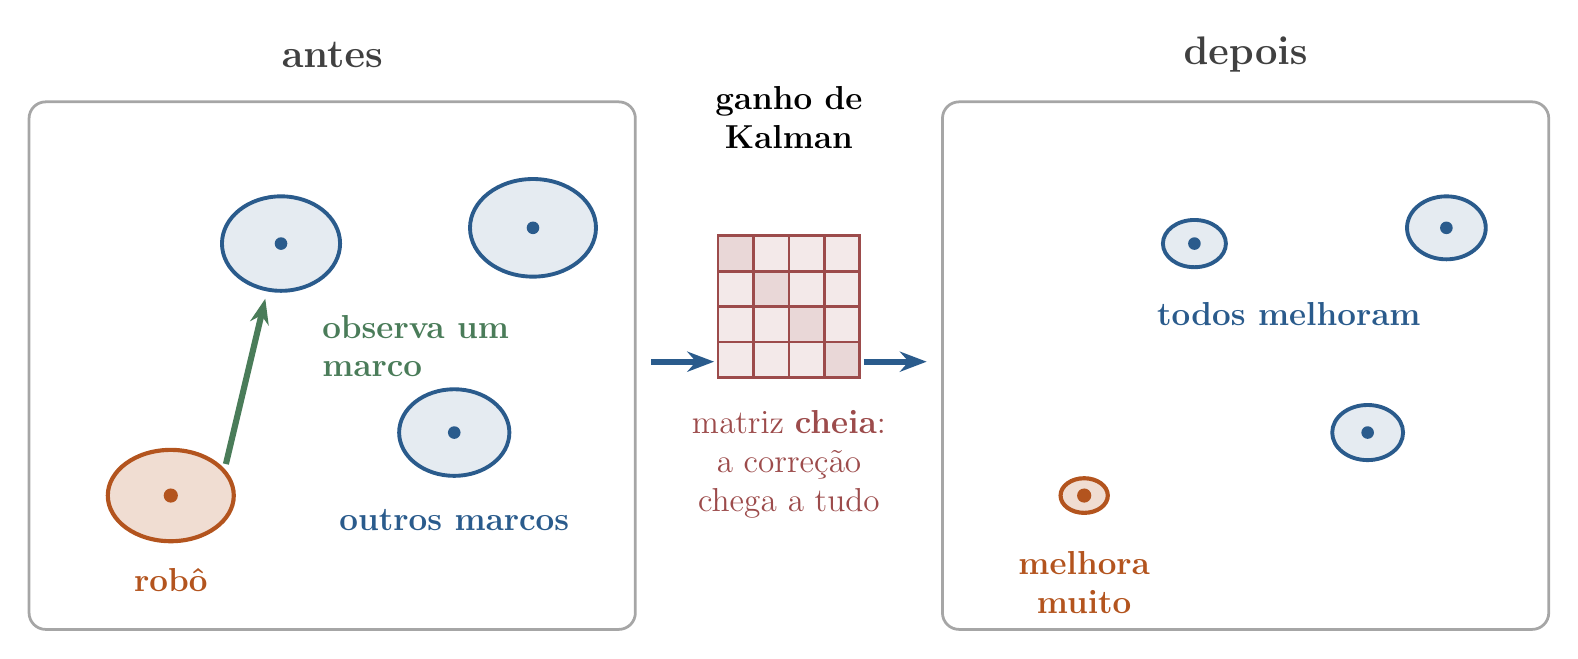
\begin{tikzpicture}[x=1cm,y=1cm]
\draw[black!35, line width=1pt, rounded corners=6pt] (0.0,0.9) rectangle (7.7,7.6);
\node[font=\Large\bfseries, black!75] at (3.85,8.2) {antes};
\draw[dblue, fill=dblue!12, line width=1.4pt] (3.2,5.8) ellipse (0.75 and 0.6); \fill[dblue] (3.2,5.8) circle (0.08);
\draw[dblue, fill=dblue!12, line width=1.4pt] (5.4,3.4) ellipse (0.7 and 0.55); \fill[dblue] (5.4,3.4) circle (0.08);
\draw[dblue, fill=dblue!12, line width=1.4pt] (6.4,6.0) ellipse (0.8 and 0.62); \fill[dblue] (6.4,6.0) circle (0.08);
\draw[dorange, fill=dorange!20, line width=1.5pt] (1.8,2.6) ellipse (0.8 and 0.58); \fill[dorange] (1.8,2.6) circle (0.09);
\draw[black!35, line width=1pt, rounded corners=6pt] (11.6,0.9) rectangle (19.3,7.6);
\node[font=\Large\bfseries, black!75] at (15.45,8.2) {depois};
\draw[dblue, fill=dblue!12, line width=1.4pt] (14.8,5.8) ellipse (0.4 and 0.3); \fill[dblue] (14.8,5.8) circle (0.08);
\draw[dblue, fill=dblue!12, line width=1.4pt] (17.0,3.4) ellipse (0.45 and 0.35); \fill[dblue] (17.0,3.4) circle (0.08);
\draw[dblue, fill=dblue!12, line width=1.4pt] (18.0,6.0) ellipse (0.5 and 0.4); \fill[dblue] (18.0,6.0) circle (0.08);
\draw[dorange, fill=dorange!20, line width=1.5pt] (13.4,2.6) ellipse (0.3 and 0.22); \fill[dorange] (13.4,2.6) circle (0.09);
\draw[dgreen, line width=2.2pt, -{Stealth[length=3.2mm]}] (2.5,3.0) -- (3.0,5.1);
\node[font=\large\bfseries, dgreen, anchor=west, text width=2.6cm] at (3.6,4.5) {observa \textbf{um} marco};
\node[font=\large\bfseries, dorange, anchor=north] at (1.8,1.8) {robô};
\node[font=\large\bfseries, dblue, anchor=north, text width=3cm, align=center] at (5.4,2.55) {outros marcos};
\node[font=\large\bfseries, dorange, text width=2.4cm, align=center] at (13.4,1.5) {melhora \textbf{muito}};
\node[font=\large\bfseries, dblue, text width=4.2cm, align=center] at (16.0,4.9) {\textbf{todos} melhoram};
\node[font=\large\bfseries, text width=3.2cm, align=center] at (9.65,7.4) {ganho de Kalman};
\draw[dtrans, line width=2.2pt, -{Stealth[length=3.4mm]}] (7.9,4.3) -- (8.7,4.3);
\draw[dtrans, line width=2.2pt, -{Stealth[length=3.4mm]}] (10.6,4.3) -- (11.4,4.3);
\draw[dred, fill=dred!22, line width=1pt] (8.75,5.9) rectangle (9.2,5.45);
\draw[dred, fill=dred!12, line width=1pt] (9.2,5.9) rectangle (9.65,5.45);
\draw[dred, fill=dred!12, line width=1pt] (9.65,5.9) rectangle (10.1,5.45);
\draw[dred, fill=dred!12, line width=1pt] (10.1,5.9) rectangle (10.55,5.45);
\draw[dred, fill=dred!12, line width=1pt] (8.75,5.45) rectangle (9.2,5.0);
\draw[dred, fill=dred!22, line width=1pt] (9.2,5.45) rectangle (9.65,5.0);
\draw[dred, fill=dred!12, line width=1pt] (9.65,5.45) rectangle (10.1,5.0);
\draw[dred, fill=dred!12, line width=1pt] (10.1,5.45) rectangle (10.55,5.0);
\draw[dred, fill=dred!12, line width=1pt] (8.75,5.0) rectangle (9.2,4.55);
\draw[dred, fill=dred!12, line width=1pt] (9.2,5.0) rectangle (9.65,4.55);
\draw[dred, fill=dred!22, line width=1pt] (9.65,5.0) rectangle (10.1,4.55);
\draw[dred, fill=dred!12, line width=1pt] (10.1,5.0) rectangle (10.55,4.55);
\draw[dred, fill=dred!12, line width=1pt] (8.75,4.55) rectangle (9.2,4.1);
\draw[dred, fill=dred!12, line width=1pt] (9.2,4.55) rectangle (9.65,4.1);
\draw[dred, fill=dred!12, line width=1pt] (9.65,4.55) rectangle (10.1,4.1);
\draw[dred, fill=dred!22, line width=1pt] (10.1,4.55) rectangle (10.55,4.1);
\node[font=\large, dred, text width=3.4cm, align=center] at (9.65,3.0) {matriz \textbf{cheia}: a correção chega a tudo};
\end{tikzpicture}
\end{document}
